% Build this document with LuaTeX, a modern Unicode-aware LaTeX engine
% that uses system TTF and OTF font files.
% This is needed for the fontspec, microtype, and nolig packages.
%
% We're using KOMA Script to hand-tune footnotes and TOC appearance.
% It should be available in your texlive distribution,
% which is how most distros package LaTeX.
\documentclass[fontsize=11pt, numbers=endperiod, draft=off]{scrbook}
% Don't draw rulers in draft mode.
\usepackage[draft=false]{scrlayer-scrpage}

% Margins: see http://practicaltypography.com/page-margins.html and
% http://practicaltypography.com/line-length.html
% We're aiming for 80-ish characters per line.
\usepackage[paperwidth=6.25in, paperheight=9.25in,
            layoutwidth=6in, layoutheight=9in,
            layouthoffset=0.125in, layoutvoffset=0.125in,
            inner=0.7in,outer=0.5in,top=0.5in,bottom=0.5in,
            includefoot,
           ]{geometry}

\usepackage{fontspec}
\usepackage[fleqn]{amsmath}

\setmainfont[
    Ligatures=TeX,
    Numbers={Proportional,Lowercase},
    % Coefficients for font-provided space, stretch, and shrink.
    % Garamond Premier is a bit tighter than Adobe Garamond,
    % but stretching it out about 20% gives about the same metrics.
    WordSpace={1.2,1.2,1},
    UprightFeatures={
        SizeFeatures={
            {Size={-10},Font=garamondpremrpro-capt},
            {Size={10-15},Font=garamondpremrpro},
            {Size={15-23},Font=garamondpremrpro-subh},
            {Size={23-},Font=garamondpremrpro-disp}
        },
    },
    BoldFeatures={
        SizeFeatures={
            {Size={-10},Font=garamondpremrpro-smbdcapt},
            {Size={10-15},Font=garamondpremrpro-smbd},
            {Size={15-23},Font=garamondpremrpro-smbdsubh},
            {Size={23-},Font=garamondpremrpro-smbddisp}
        },
    },
    ItalicFeatures={
        SizeFeatures={
            {Size={-10},Font=garamondpremrpro-itcapt},
            {Size={10-15},Font=garamondpremrpro-it},
            {Size={15-23},Font=garamondpremrpro-itsubh},
            {Size={23-},Font=garamondpremrpro-itdisp}
            },
    },
    BoldItalicFeatures={
        SizeFeatures={
            {Size={-10},Font=garamondpremrpro-smbditcapt},
            {Size={10-15},Font=garamondpremrpro-smbdit},
            {Size={15-23},Font=garamondpremrpro-smbditsubh},
            {Size={23-},Font=garamondpremrpro-smbditdisp}
        },
    },
]{Garamond Premier Pro}
\setsansfont[Ligatures=TeX,
             Scale=MatchUppercase,
             Style=Alternate, % Straight-legged R
             UprightFont = *-55Rg,
             ItalicFont = *-56It,
             BoldFont = *-65Md,
             BoldItalicFont = *-66MdIt
             ]{NHaasGroteskTXPro}
\setmonofont[Scale=MatchLowercase]{mononoki}

% We'll be using this quite a bit:
\newfontfamily{\lm}[%
    Ligatures=TeX,
    SmallCapsFont = * Caps
]{Latin Modern Roman}

\usepackage{polyglossia}
\setdefaultlanguage[variant=american]{english}
\setotherlanguage{french}

\usepackage{microtype} % Font expansion, protrusion, and other goodness

% Disable ligatures across grapheme boundaries
% (see the package manual for details.)
\usepackage[american]{selnolig}
% I have no idea why Garamond has this on by default.
\nolig{Th}{T|h}

% Use symbols for footnotes, resetting each page
\usepackage[perpage,bottom,symbol*]{footmisc}

% Left flush footnotes. See the KOMA Script manual.
\deffootnote[1em]{1em}{1em}{\thefootnotemark}
% Set the width of the rule separating body text and footnotes
\setfootnoterule{0.8\textwidth}

% Like many fonts, Equity's asterisk is already set in a "superscripted" form.
% Superscripting *that* makes it annoyingly small.
% To fix this, we have to redefine footnote marks so that they aren't superscript,
% then raise all the other symbols.
%
% Feel free to remove this if your body type doesn't have this peculiarity,
% but unfortunately many do.
% See http://tex.stackexchange.com/a/16241
%
% We use the Unicode symbols themselves (instead of \dagger, \ddagger, \P, etc.)
% because the latter fall back to Computer Modern/Latin Modern in some cases,
% (e.g., if you're using mathastext instead of unicode-math).
% Alternatively, you could use \textdagger, \textddagger, etc.,
% but this seems more concise.
\DefineFNsymbols*{tweaked}{%
    {*}%
    {\textsuperscript†}%
    {\textsuperscript‡}%
    {\textsuperscript{◊}}%
    {\textsuperscript{§}}%
    {**}%
    {\textsuperscript{††}}%
    {\textsuperscript{‡‡}}%
}
\setfnsymbol{tweaked}
\deffootnotemark{\thefootnotemark}

\DeclareTOCStyleEntry[%
    beforeskip=8pt,
    entryformat = \bfseries,
    entrynumberformat = \addfontfeature{Numbers={Tabular,Uppercase}},
    pagenumberformat = \addfontfeature{Numbers={Tabular,Uppercase}},
    linefill = \TOCLineLeaderFill
]{tocline}{chapter}
\DeclareTOCStyleEntry[%
    beforeskip=1pt,
    entrynumberformat = \addfontfeature{Numbers={Tabular,Uppercase}},
    pagenumberformat = \addfontfeature{Numbers={Tabular,Uppercase}},
    indent=0.4in
]{tocline}{section}
\DeclareTOCStyleEntry[%
    beforeskip=0pt,
    entrynumberformat = \addfontfeature{Numbers={Tabular,Uppercase}},
    pagenumberformat = \addfontfeature{Numbers={Tabular,Uppercase}},
    indent=0.6in
]{tocline}{subsection}

% Don't use a sans font for description labels.
\addtokomafont{descriptionlabel}{\rmfamily}
% Sections and such use serif type.
\setkomafont{disposition}{\rmfamily}
% Uppercase numbers for chapters.
\addtokomafont{chapter}{\addfontfeature{Numbers=Uppercase}}
% Set size and style of section and subsections
\setkomafont{section}{\Large\itshape}
\setkomafont{subsection}{\large\itshape}
% Don't put big spaces before chapter headings
\RedeclareSectionCommand[beforeskip=0.15in]{chapter}

\setcapwidth[c]{.75\textwidth}
%\setcapmargin{0pt}
\setkomafont{caption}{\sffamily\footnotesize}
\setkomafont{captionlabel}{\sffamily\footnotesize}
\renewcommand*{\figureformat}{}
\renewcommand*{\tableformat}{}
\renewcommand*{\captionformat}{}

% Use uppercase numbers for numbered lists.
% (We're using lowercase ones for the body text.)
% See http://tex.stackexchange.com/a/133186
\usepackage{enumitem}
\setlist[enumerate]{font=\addfontfeatures{Numbers=Uppercase}}
\setlist[description]{leftmargin=1em}

\usepackage{tabularx}

% Custom footer
\usepackage{scrlayer-scrpage}
\clearpairofpagestyles
\pagestyle{scrheadings}
\setkomafont{pagefoot}{\upshape}
\lefoot*{\thepage} % \, is a TeX primitive for a thin space.
\rofoot*{\thepage} % \, is a TeX primitive for a thin space.

\usepackage{changepage} % For adjustwidth

\usepackage{mflogo} % for METAFONT
\usepackage{metalogo} % for \LuaLaTeX

\usepackage{multicol}

\usepackage{endnotes}
% Endnotes _mostly_ works... with Koma Script, no less.
% I suppose I can only grumble a little about the hackery below.
\renewcommand\enoteheading{\chapter{Notes}}
\renewcommand\enoteformat{\leavevmode\llap{\makeenmark}}
% OTF goodness...
\renewcommand\makeenmark{{\addfontfeature{VerticalPosition=Superior}\theenmark}}

\usepackage{listings}
\lstset
{
    language=[LaTeX]TeX,
    breaklines=false,
    basicstyle=\ttfamily\small,
    keywordstyle=\ttfamily\small,
    commentstyle=\ttfamily\small,
}

\newenvironment{leftfigure}
  {\par\vspace{0.5\baselineskip minus 0.3\baselineskip}\begin{adjustwidth}{1.5em}{0pt}}
  {\end{adjustwidth}\vspace*{0.5\baselineskip minus 0.3\baselineskip}}

\newenvironment{centerfigure}
  {\par\vspace{0.5\baselineskip minus 0.3\baselineskip}\begin{adjustwidth}{1.5em}{1.5em}\centering}
  {\end{adjustwidth}\vspace*{0.5\baselineskip minus 0.3\baselineskip}}

\usepackage{graphicx}

\usepackage{csquotes}

\title{Modern LaTeX}
\author{Matt Kline}
\date{\today}

% Custom footer
% Hyperlinks
\usepackage[unicode,pdfusetitle,hidelinks]{hyperref}

% Use \punckern to overlap periods, commas, and footnote markers
% for a tighter look.
% Care should be taken to not make it too tight - f" and the like can overlap
% if you're not careful.
\newcommand{\punckern}{\kern-0.2ex}
% For placing commas close to, or under, quotes they follow.
% We're programmers, and we blatantly disregard American typographical norms
% to put the quotes inside, but we can at least make it look a bit nicer.
\newcommand{\quotekern}{\kern-0.5ex}


% Create an unbreakable string of text in a monospaced font.
% Useful for `command --line --args`
\newcommand{\monobox}[1]{\mbox{\texttt{#1}}}

\newcommand{\otffrac}[2]{\mbox{%
    {\addfontfeature{VerticalPosition=Superior}#1}%
    ^^^^2044% Unicode fraction slash
    {\addfontfeature{VerticalPosition=Inferior}#2}%
}}
\newcommand{\otford}[2]{\mbox{%
    {\addfontfeature{Numbers=LowercaseOff}#1}%
    {\addfontfeature{VerticalPosition=Superior}#2}%
}}

% C++ looks nicer if the ++ is in a monospace font and raised a bit.
% Also, use uppercase numbers to match the capital C.
\newcommand{\plusplus}{\raisebox{0.1ex}{++}}
\newcommand{\cpp}[1]{C\kern-0.1ex\plusplus{\addfontfeature{Numbers=LowercaseOff}#1}}

% Italicize new terms
\newcommand{\introduce}[1]{\textit{#1}}

% Letterspace acronyms a bit.
\newcommand{\acronym}[1]{\textsc{\addfontfeature{LetterSpace=6}#1}}

% "Chapter <num>" references
\newcommand{\chapref}[1]{%
    {\addfontfeature{Numbers={Proportional,Uppercase}}Chapter~\ref{#1}}%
}

% monospace URLs (without setting the http://...)
\newcommand{\http}[1]{\href{http://#1}{\texttt{#1}}}
\newcommand{\https}[1]{\href{https://#1}{\texttt{#1}}}

% See http://tex.stackexchange.com/a/68310
\makeatletter
\let\runauthor\@author
\let\rundate\@date
\let\runtitle\@title
\makeatother

% Spend a bit more time to get better word spacing.
% See http://tex.stackexchange.com/a/52855/92465
\emergencystretch=1ex

% Do as I say, not as I do.
\widowpenalty=10000
\clubpenalty=10000

\begin{document}
\fontsize{11pt}{13pt}\selectfont

\frontmatter
\setcounter{secnumdepth}{0}
\setlength\parindent{0pt}

% Custom title instead of \maketitle
\pagenumbering{gobble}
\vspace*{1.5in}
\begin{center}
\fontsize{0.5in}{0.7in}\selectfont
Modern

\fontsize{1in}{1.1in}\selectfont
\LaTeX
\vfill
\LARGE
Matt Kline
\end{center}
\clearpage

\null
\vfill
Some crappy draft, typeset \today.
\vspace*{0.5in}

The author apologizes for any typos, misattributions, and other flubs.
He welcomes you to point them out on this book's Github
repository at \\
\https{github.com/mrkline/latex-book} \\
Questions, comments, concerns, and diatribes can also be sent to \\
\texttt{matt <at> bitbashing.io}

The author does not have a checking account with the Bank of San Serriffe,
but will happily compensate your feedback with a beverage of your choice the
next time we meet.

\vspace*{0.5in}
{\addfontfeature{Numbers={Proportional,Uppercase}}
Copyright © 2018 \\
by \runauthor
\bigskip

This book is licensed under the \\
Creative Commons Attribution-ShareAlike~4.0 International License. \\
The license's full text is available at \\
\https{creativecommons.org/licenses/by-sa/4.0/legalcode}
}
\clearpage

\vspace*{1in}
{\itshape%
%\noindent To Donald, Leslie, \\
%Ellen, Erik, Jost, Matthew, \& Robert
%\bigskip
%
To Max, who once told me about a cool program he used to type up
his college papers.
}
\cleardoublepage

\pagenumbering{roman}
\tableofcontents

\mainmatter
\setlength\parindent{1em}

\pagenumbering{arabic}
\setcounter{page}{1} % Restart page numbering after the ToC.
\cleardoublepage

\chapter{\texorpdfstring{\LaTeX}{LaTeX}?}

\LaTeX{} is a program\footnote{And a markup language,
and (sort of) a programming language, and a bit of a cult.
But that's all for later.}
for crafting written documents, like papers, presentations,
or even the book you're reading right now.
In some sense, it's an alternative to the likes of Microsoft Word,
Apple Pages, Google Docs, or LibreOffice Writer.

Unlike these other applications, which work on the principle of
\introduce{What You See Is What You Get} \acronym{(wysiwyg)},
\LaTeX{} documents are built from a ``plain'' text file,
using \introduce{markup} to specify how things should look.
When you are ready, \LaTeX{} generates your document from this file
based on the formatting rules you gave it.
If you've done any web development, this is a similar process---just
as \acronym{html} and \acronym{css} describe the page you want
browsers to draw, your markup describes the appearance of your
document to \LaTeX.

\begin{leftfigure}
\begin{lstlisting}
Unlike these other applications, which work on the principle of
\introduce{What You See Is What You Get} \acronym{(wysiwyg)},
\LaTeX{} documents are built from a ``plain'' text file,
using \introduce{markup} to specify how things should look.
When you are ready, \LaTeX{} generates your document from this file
based on the formatting rules you gave it.
If you've done any web development, this is a similar process---just
as \acronym{html} and \acronym{css} describe the page you want
browsers to draw, your markup describes the appearance of your
document to \LaTeX.
\end{lstlisting}
\captionof{figure}{The \LaTeX{} markup for the above paragraph}
\end{leftfigure}

This might seem alien to you if you've never worked with a markup system before.
However, it comes with a few advantages:
\begin{enumerate}
\item You can handle a document's contents and its presentation separately.
    At the beginning of each document,
    you describe the design you want.
    From there, \LaTeX{} handles the rest for you,
    keeping fonts, sizes, line heights,
    and other layout considerations consistent across your whole text.
    Compare this to a \acronym{wysiwyg} system,
    where you must constantly concern yourself with your work's appearance
    as you write.
    If you changed the look of a caption,
    did you make sure to find all the other captions and do the
    same?\footnote{This isn't to say that it's impossible
    to create nice, consistent documents with \acronym{wysiwyg} tools.
    Many of them have gotten much better at automating these sorts of
    tasks in recent years.}
    If the program formats something in a way you don't like,
    how hard is it to fix?%\footnote{I spent far too much of my childhood
    %fighting with Word about how it wrapped text around images.}

\item You can define your own rules, then tweak them to immediately change
    everywhere they're used in your document.
    For example, the \verb|\introduce| and \verb|\acronym| commands you saw above
    are my own creations. The former \introduce{italicizes} text, and
    the latter sets words in \acronym{small caps} with a bit of extra
    \,\textsc{\addfontfeature{LetterSpace=15}letterspacing}\, so the characters
    don't look \textsc{too crowded}.
    If I wake up tomorrow and decide to introduce new terms
    \textbf{\itshape with this look} and set acronyms
    {\small\addfontfeature{LetterSpace=8} LIKE THIS},
    I just change the two lines that define those commands
    to update every place in the book that uses them.
\item In \LaTeX, the document's structure is immediately visible
    and can be easily copied.
    In \acronym{wysiwyg} systems, it is often unobvious
    how certain formatting was produced
    or how to replicate it.
\item Since the document source is plain text,
    \begin{itemize}
    \item It can be read and understood with any text editor.
    \item Content can be easily generated programmatically.
    \item Changes are easily tracked with version control software.
    \end{itemize}
\end{enumerate}

This is all well and good,
but misses the main selling point of \LaTeX.
You should try it because you care about\ldots

\chapter{Typography}
\label{typography}

Modern life is a constant battle for your time---every day,
dozens of ads, apps, emails, sites, and texts fight
for a few short minutes of it.
To put ideas into the world,
nothing is more important than catching and holding
the attention of your audience.
Typography is a tool to do so---a good design doesn't ``look nice''
only for the sake of art---it draws readers in.\punckern\endnote{Matthew Butterick,
``Typography for Docs''
(presented at the Write The Docs Conference, April 8, 2013),
\url{https://www.youtube.com/watch?v=8J6HuvosP0s}}
%Matthew Butterick's \textit{Practical Typography} calls it
%``the visual component of the written word.\quotekern''
It sets their expectations and establishes a subliminal ``brand'' for your
work.\punckern\endnote{Erik Spiekermann, ``Type is Visible Language''
(presented at Beyond Tellerrand, Düsseldorf, Germany, May 19--21, 2014),
\url{https://www.youtube.com/watch?v=ggQpDu63kk0}}
It's the \emph{how} of text.
\begin{leftfigure}
\fontspec{TeX Gyre Termes}\fontsize{12pt}{24pt}\selectfont\raggedright
Typography is why this reminds you of the terrible essays
you wrote in school.
Would you like to read an entire book this way?
\end{leftfigure}
It is why
\begin{leftfigure}
\noindent\fontspec{FuturaCon-ExtBol}\Large DO IT LATER
\end{leftfigure}
seems oddly reminiscent of a certain shoe company's advertising,
or how
\begin{center}
\fontspec[Ligatures=TeX, Scale=MatchLowercase]{Futura-Med}
\noindent MEN FROM THE PLANET EARTH \\
FIRST SET FOOT UPON THE MOON \\
JULY 1969, A.~D.
\end{center}
Typography shows people
what you have to say before they read a single word.

This is where \LaTeX{} shines, and
unless you want to give Adobe large sums
of money for InDesign or InCopy,
you won't find any better typesetting software.
By carefully handling subtle details---like how words are spaced,
hyphenated, and arranged into lines---\LaTeX{} provides high-quality layout
with relatively little effort from you, the author.
Modern versions can also take advantage of new\footnote{By new,
I mean ``from the mid-1990s''\quotekern, but web browsers and desktop publishing
software are only just starting to catch up.} advances in computer typography,
giving you the same tools available to professional designers and publishers.

\chapter{Another Guide?}

One might wonder why the world needs another \LaTeX{} guide.
After all, it's been out for more than 30 years.
A quick Amazon search finds nearly a dozen books on the topic.
There are plenty of great resources online.

Unfortunately, most guides have two fatal flaws: they are long,
and they are old.
The first is anathema to newcomers---if somebody asks about \LaTeX{},
throwing a 200+ page book at them isn't an encouraging start.
The second matters because of how much the world of computer typesetting has
changed since 1986.

When \LaTeX{} was first released that year, none of the publishing technologies
we use today existed.
Adobe wouldn't introduce their Portable Document Format for another seven years,
and home computers wouldn't support it ubiquitously for several more.
Digital typography was a new field, and desktop publishing was \emph{just}
getting off the ground.\punckern\endnote{\textit{Graphic Means:
A History of Graphic Design Production}, directed by Briar Levit (2017)}
This shows---badly---in most \LaTeX{} guides.
If you look for instructions to change your document's font,
you'll likely get swamped with bespoke nonsense.\punckern\footnote{%
Take all criticisms of \LaTeX's past here with a grain of
salt. After all, the fact that all of the technology around it became
obsolete---multiple times---is a testament to its staying power.}

The good news is that  \LaTeX{} has improved by leaps and bounds in recent years.
It's time for a guide that doesn't weigh you down with decades of legacy.
It's also time for one that doesn't try to be some comprehensive reference.
After all, you're a smart, resourceful individual who knows how to use a search
engine.
This book will:
\begin{enumerate}
\item Teach you the very basics of using \LaTeX.
\item Point you to places where you can learn more.
\item Show you how to use modern technologies like OpenType and microtypography
    to create professional-quality documents.
\item End promptly thereafter.
\end{enumerate}
Let's begin.


\chapter{Installation}
\label{installation}

You install \LaTeX{} on your computer by downloading a \introduce{distribution},
which comes with:
\begin{enumerate}
\item \LaTeX, the program---the thing that turns text files into typeset
    documents.\footnote{We'll actually be installing multiple \LaTeX{} programs,
    but we're getting to that.}
\item A common set of \LaTeX{} \introduce{packages}.
    Packages are pieces of code that can be placed in your documents to
    do all sorts of things, like change their style or add new commands.
    We'll see lots of them in action throughout this book.
\item Miscellaneous tools, such as editors.
\end{enumerate}
Each major operating system has its own \LaTeX{} distribution:
\begin{description}
\item[Mac OS] has Mac\TeX. Grab it from \http{www.tug.org/mactex}
    and follow the instructions there to install it.

\item[Windows] has Mik\TeX.
    Install it from \https{miktex.org/download}.
    Mik\TeX{} offers the unique ability to automatically download
    additional packages if your document uses one that it can't find
    on your computer.

\item[Linux and BSD] use \TeX{} Live.
    Like most software, this is provided through your
    \acronym{os}'s package manager.
    Linux distributions usually contain a \texttt{texlive-\allowbreak full}
    or \texttt{texlive-\allowbreak most} package that installs everything
    you need.\punckern\footnote{%
    If you'd rather keep the install size down,
    Linux distributions usually break \TeX{} Live into multiple distro packages.
    Look for ones with names like
    \texttt{texlive-\allowbreak core}, \texttt{texlive-\allowbreak luatex}
    and \texttt{texlive-\allowbreak xetex}.
    As you work with \LaTeX, you may need less-common packages,
    which usually have names like \texttt{texlive-\allowbreak latexextra},
    \texttt{texlive-\allowbreak science}, and so on.
    Of course, all of this may vary from one Linux distribution to another.}
\end{description}

\section{Editors}

Since \LaTeX{} source files are regular text files,
you're free to create them with the usual choices of Vim, Emacs,
Sublime, Notepad\plusplus, and so on.\punckern\footnote{If you have never used
any of these, try a few.
They're popular among programmers and other folks who shuffle text around
screens all day. Just don't use Notepad. Life is too short.}
However, there are also editors designed specifically for \LaTeX{},
which often come with their own built-in \acronym{pdf} viewer.
You can find a fairly comprehensive list on the \LaTeX{} Wikibook,
in its installation chapter. (See Appendix~\ref{resources}.)

\section{Online options}

If you'd rather not install \LaTeX{} on your computer,
you can try online editors such as Share\LaTeX{} and Overleaf.
This book won't focus on these web-based tools,
but almost all of the same basics apply.
(Of course, you have less control over certain aspects of online versions,
such as available fonts, the version of \LaTeX{} that's used, and so on.)


\chapter{Hello, \texorpdfstring{\LaTeX}{LaTeX}!}

Now that you have a \LaTeX{} distribution installed,
let's try it out.
Open up your editor of choice and save the following as \texttt{hello.tex}:
\begin{leftfigure}
\begin{lstlisting}
\documentclass{article}
% Say hello
\begin{document}
Hello, World!
\end{document}
\end{lstlisting}
\end{leftfigure}
We then run this file through \LaTeX{} (the program)\footnote{Not to be
confused with \LaTeX{} the lunchbox, \LaTeX{} the breakfast cereal,
or \LaTeX{} the flamethrower. The kids love this stuff!}
to get our document.
The installation places several different versions---or
\introduce{engines}---on your machine,
but for the entire book, we'll always use \LuaLaTeX{} or \XeLaTeX.
These are the newest engines available---see Appendix~\ref{history} for an
explanation of how they differ from the others.

If you are using a \LaTeX{}-specific editor, it may contain a drop-down menu
or some other configuration to select the engine you'd like to use,
as well as a button to generate your document.
Otherwise, from a terminal,\punckern\footnote{How to work a terminal emulator,
making sure the newly-installed \LaTeX{} programs are in your \texttt{PATH},
and so on are all outside the scope of this book.
As is tradition, the leading dollar sign in examples just denotes a console
prompt, and shouldn't actually be typed.}
run the following:
\begin{leftfigure}
\begin{lstlisting}
$ xelatex hello.tex
\end{lstlisting}
\end{leftfigure}
Feel free to use \texttt{lualatex} instead---there are a few differences
between the two, but either is fine for now.
With luck, you should see some output that ends in a message like:
\begin{leftfigure}
\begin{lstlisting}
Output written on hello.pdf (1 page).
Transcript written on hello.log.
\end{lstlisting}
\end{leftfigure}
and in your current directory, a newly minted \texttt{hello.pdf}.
Open it up and you should find a page with this at the top:
\begin{leftfigure}
\lm Hello, World!
\end{leftfigure}
Congrats,
you just created your first document!

Let's unpack what we did.
All \LaTeX{} documents begin with a \verb|\documentclass| declaration,
which picks a style to use.
Many classes are available---and you can even create your own---but common
ones include \texttt{article}, \texttt{report}, \texttt{book},
and \texttt{beamer}.\punckern\footnote{This last one is for slideshows.
Kind of an odd name, no?}
For your average document, \texttt{article} is probably a good choice.
Next is, \verb|% Say hello|.
This is a \introduce{comment}---anything placed after a percent symbol on a line
is ignored by the engine,
so we can use \verb|%| to leave notes about what's going on to anybody reading
the document's source.\punckern\footnote{Including, perhaps most importantly,
a confused version of your future self!}
Finally, we use \verb|\begin{document}| to tell \LaTeX{} that what follows
is our actual contents,
and we use \verb|\end{document}| to state that we are finished.

So far, so good.
Let's cover some more basics.

\section{Spacing}

\LaTeX{} generally handles inter-word spacing for you, regardless of how many
spaces\footnote{Or tabs} you type. For example,
\begin{leftfigure}
\begin{lstlisting}
The number  of   spaces    between words doesn't   matter. The same
is true for sentences.

An empty line starts a new paragraph.
\end{lstlisting}
\end{leftfigure}
yields
\begin{leftfigure}
\lm The number  of   spaces    between words doesn't   matter. The same
is true for sentences.

An empty line  starts a new paragraph.
\end{leftfigure}
Notice that \LaTeX{} is automatically following typographic
conventions, such as indenting new paragraphs and leaving more space after a
period than it leaves between words.
One quirk to be aware of is that comments ``eat'' all of the leading
space on the subsequent line, such that
\begin{leftfigure}
\begin{lstlisting}
This% weird, right?
  is strange
\end{lstlisting}
\end{leftfigure}
gives
\begin{leftfigure}
This% weird, right?
  is strange
\end{leftfigure}

\section{Commands}

\LaTeX{} has various commands to issue instructions to
the engine, and you can define your own as well.
Their names always begin with a backslash (\,\texttt{\textbackslash}\,),
contain only letters, and are case-sensitive.\punckern\footnote{%
% \verb doesn't play nicely in footnotes, so...
\texttt{\textbackslash foo}
is different from \texttt{\textbackslash Foo}, for example.}
Some commands require parameters, or \introduce{arguments}---\verb|\documentclass|,
for example, needs to know which document class we want.
These arguments are enclosed in subsequent pairs of braces,
so if some command needed two arguments, we would type:
\begin{leftfigure}
\begin{lstlisting}
\somecommand{argument1}{argument2}
\end{lstlisting}
\end{leftfigure}
Many commands also take optional arguments, which are enclosed in square
brackets and precede the mandatory ones.
Say you want to inform \LaTeX{} that your document will be printed as
double-sided pages.\punckern\footnote{\texttt{twoside} introduces commands
that only make sense in the context of double-sided printing,
such as ones that skip to the start of the next odd page.
It also allows you to have different margins for even and odd pages,
which is useful for texts like this book.}
This is done with an optional argument to \verb|\documentclass|:
\begin{leftfigure}
\begin{lstlisting}
\documentclass[twoside]{article}
\end{lstlisting}
\end{leftfigure}

Other commands take no arguments at all, such as \verb|\LaTeX|,
which prints the \LaTeX{} logo.
Know that these commands consume any space that follows them.
For example,
\begin{leftfigure}
\begin{lstlisting}
\LaTeX is great, but it can be strange sometimes.
\end{lstlisting}
\end{leftfigure}
will give you
\begin{leftfigure}
\lm \LaTeX is great, but it can be strange sometimes.
\end{leftfigure}
You can fix this by adding an empty pair of braces to the command.
Of course, the braces aren't needed if there is no space to preserve:
\begin{leftfigure}
\begin{lstlisting}
Let's learn \LaTeX! \LaTeX{} is a powerful tool,
but a few of its rules are a little weird.
\end{lstlisting}
\end{leftfigure}
gets us
\begin{leftfigure}
\lm Let's learn \LaTeX! \LaTeX{} is a powerful tool,
but a few of its rules are a little weird.
\end{leftfigure}

\section{Special characters and line breaks}

Some characters have special meanings in \LaTeX.
We saw above, for example, that \verb|%| starts a comment
and \verb|\| starts a command.
The full list of special characters is:
\begin{leftfigure}
\begin{lstlisting}
# $ % ^ & _ { } ~ \
\end{lstlisting}
\end{leftfigure}
All have corresponding commands
if you want to make them appear in your document:
\begin{leftfigure}
\begin{lstlisting}
\# \$ \% \^{} \& \_ \{ \} \~{} \textbackslash
\end{lstlisting}
\end{leftfigure}
will produce
\begin{leftfigure}
\lm \# \$ \% \^{} \& \_ \{ \} \~{} \textbackslash
\end{leftfigure}
Regardless of what comes after them, you must always add braces to
the caret (\,\texttt{\^{}}\,) and tilde (\,\~{}\,).
This is a relic from days when these characters were used to produce
\introduce{diacritical marks}:
once upon a time, users had to typeset ``jalapeño'' as
\verb|jalape\~no|.
Today, we just type \texttt{ñ} into our source
file.\punckern\footnote{The ease with which you can do this depends
on the keyboard you're using, the language settings in your \acronym{os},
and your editor.
Later on, we'll talk much more about non-English languages and Unicode fun.}

If you're wondering why we print \texttt{\textbackslash} with
\verb|\textbackslash| instead of just \verb|\\|,
it's because the latter is the command to force a line break.
\begin{leftfigure}
\begin{lstlisting}
Give me \\
a brand new line!
\end{lstlisting}
\end{leftfigure}
obeys:
\begin{leftfigure}
\lm Give me \\
a brand new line!
\end{leftfigure}
Use this power judiciously---deciding how to break paragraphs into lines
automatically is one of \LaTeX{}'s best skills.

\section{Environments}

We often control our document by organizing text into \introduce{environments}.
These always start with \verb|\begin{name}| and conclude with \verb|\end{name}|,
where \texttt{name} is that of the environment.
Take \texttt{quote}, which adds additional spacing on both sides of a block
quotation:
\begin{leftfigure}
\begin{lstlisting}
Donald Knuth once wrote,
\begin{quote}
We should forget about small efficiencies,
say about 97\% of the time:
premature optimization is the root of all evil.
Yet we should not pass up our opportunities in that critical 3\%.
\end{quote}
\end{lstlisting}
\end{leftfigure}
gives us
\begin{leftfigure}
\lm
Donald Knuth once wrote,
\begin{quote}
We should forget about small efficiencies,
say about 97\% of the time:
premature optimization is the root of all evil.
Yet we should not pass up our opportunities in that critical 3\%.
\end{quote}
\end{leftfigure}

\section{Groups and command scope}
Some commands change how \LaTeX{} typesets the following text.
\verb|\itshape|, for example, \textit{italicizes} everything that comes after it.
If we want to limit a command's effect to a certain region, we can surround it
with braces.
\begin{leftfigure}
\begin{lstlisting}
{\itshape Sometimes we want italics}, but only sometimes.
\end{lstlisting}
\end{leftfigure}
is set as
\begin{leftfigure}
\lm {\itshape Sometimes we want italics}, but only sometimes.
\end{leftfigure}
The text within the braces forms a \introduce{group},
and all commands issued inside the group only take effect until it ends.
Environments also also form implicit groups:
\begin{leftfigure}
\begin{lstlisting}
\begin{quote}
\itshape If I italicize a quote, the following text will
use upright type again.
\end{quote}
See? Back to normal.
\end{lstlisting}
\end{leftfigure}
produces
\begin{leftfigure}
\lm
\begin{quote}
\itshape If I italicize a quote, the following text will
use upright type again.
\end{quote}
See? Back to normal.
\end{leftfigure}
One final use of groups is to get around the spacing oddities of zero-argument
commands: some prefer \verb|{\LaTeX}| over \verb|\LaTeX{}|.


\chapter{Document Structure}
\label{structure}

Every \LaTeX{} document is different,
but all share a few common elements.

\section{Packages and the preamble}
In the last chapter, you saw:
\begin{leftfigure}
\begin{lstlisting}
\documentclass{article}

\begin{document}
Hello, World!
\end{document}
\end{lstlisting}
\end{leftfigure}
The area between the \verb|\documentclass| command and the start of the
\texttt{document} environment is called the \introduce{preamble}.
Here, we perform any setup we need---such as importing packages
and defining commands---to control how our document
will look.

As mentioned in \chapref{installation},
\introduce{packages} contain code to modify your document in interesting ways.
The ones found in your \LaTeX{} distribution come from the Comprehensive \TeX{}
Archive Network, or \acronym{ctan},\punckern\footnote{Curious readers may
be wondering what \TeX{} is, and how it differs from \LaTeX.
The short version is that \TeX{} is the typesetting system that \LaTeX{}
is built on top of---the latter is a framework of commands for the former.
(For example, \texttt{\textbackslash documentclass} and friends are provided by
\LaTeX{}, but the \TeX{} engine is what's actually laying out your document.)
The long version is at the back of this book as Appendix~\ref{history}.
We won't discuss how to use plain \TeX{} here. That's for another book---the
\TeX book.}
at \https{ctan.org}.
Package manuals are also found there,
so make it your first stop when learning how to use one.

To import a package, add a \verb|\usepackage| command,
with the package's name as its argument.
As a simple example, let's write a document with the \texttt{metalogo}
package, which adds \verb|\LuaLaTeX| and \verb|\XeLaTeX|:
\begin{leftfigure}
\begin{lstlisting}
\documentclass{article}

\usepackage{metalogo}

\begin{document}
\XeLaTeX{} and \LuaLaTeX{} are neat.
\end{document}
\end{lstlisting}
\end{leftfigure}
\begin{samepage}
should get you a \textsc{pdf} that reads
\begin{leftfigure}
\lm \XeLaTeX{} and \LuaLaTeX{} are neat.
\end{leftfigure}
\end{samepage}
Like other commands, \verb|\usepackage| accepts optional arguments.
The \texttt{geometry} package, for instance,
takes your desired paper size and margins.
For \acronym{us}~\textsc{l}etter paper with one-inch margins,
you type:\footnote{Notice
that command arguments can be spaced in whatever way is most convenient to you,
so long as there are no empty lines between arguments.}
\begin{leftfigure}
\begin{lstlisting}
\usepackage[letterpaper,
            left=1in, right=1in, top=1in, bottom=1in
           ]{geometry}
\end{lstlisting}
\end{leftfigure}

\section{Titles, sections, and other hierarchy}

Authors often split their works into sections to help readers navigate them.
\LaTeX{} offers seven different commands to break up your documents:
\verb|\part|, \verb|\chapter|, \verb|\section|, \verb|\subsection|,
\verb|\subsubsection|, \verb|\paragraph|, and \verb|\subparagraph|.
To use one, issue the command where you want that section to start,
providing its name as the argument.
For example,
\begin{leftfigure}
\begin{lstlisting}
\documentclass{book}

\begin{document}
\chapter{The Start}
This is a very short chapter in a very short book.

\chapter{The End}
Is the book over yet?

\section{No!}
There's some more we must do before we go.

\section{Yes!}
Goodbye!
\end{document}
\end{lstlisting}
\end{leftfigure}
Some levels are only available in certain document classes---chapters,
for example, only appear in books.
And don't go too crazy with these commands.
Most works only benefit from a few levels of hierarchy.

Sections\footnote{By this I mean all levels, not just
\texttt{\textbackslash section}.}
are automatically numbered---for example,
the title of this chapter was produced with \verb|\chapter{Document Structure}|,
and \LaTeX{} figured out that it was chapter~\ref{structure}.

\section{What next?}

As promised, this book isn't a comprehensive reference,
but it \emph{will} point you to places where you can learn more.
We'll wrap up most chapters with a list of related topics you could
explore next.

Consider learning how to:
\begin{itemize}
\item Automatically start your document with its title, the author's name,
    and the date using \verb|\maketitle|.
\item Have \LaTeX{} build you a table of contents
    with \verb|\tableofcontents|.
\item Control section numbering with \verb|\setcounter{secnumdepth}|
and starred section commands, e.g., \verb|\subsection*{foo}|.
\item Create auto-updating cross-references with \verb|\label| and \verb|\ref|.
\item Use KOMA~Script, a set of document classes and packages
that make it easy to customize nearly every aspect of your document,
from heading fonts to footnotes.
\item Include images with the \texttt{graphicx} package.
\item Add hyperlinks to your \acronym{pdf} with the \texttt{hyperref} package.
\item Split large documents into multiple files using \verb|\input|.
\end{itemize}


\chapter{Formatting Text}

\section{Emphasis}

\section{Sizes}

The default text size is controlled by your document class.
It is usually ten points,\punckern\footnote{In most digital publishing,
one point is \otffrac{1}{72} of an inch.
In \LaTeX{}, for historical reasons, it is
\otffrac{100}{7227} of an inch.}
but this can be adjusted by passing additonal arguments to
\verb|\documentclass|.\punckern\footnote{The standard \LaTeX{} classes accept
\texttt{10pt}, \texttt{11pt}, or \texttt{12pt}.
KOMA Script classes accept arbitrary sizes with
\monobox{fontsize=<size>}.}
To scale text relative to this size, use the following commands:
\begin{leftfigure}
\lm
\renewcommand{\arraystretch}{1.5}
\begin{tabular}{l l}
\verb|\tiny| & \tiny Example Text \\
\verb|\scriptsize| & \scriptsize Example Text \\
\verb|\footnotesize| & \footnotesize Example Text \\
\verb|\small| & \small Example Text \\
\verb|\normalsize| & \normalsize Example Text \\
\verb|\large| & \large Example Text \\
\verb|\Large| & \Large Example Text \\
\verb|\LARGE| & \LARGE Example Text \\
\verb|\huge| & \huge Example Text \\
\verb|\Huge| & \Huge Example Text \\
\end{tabular}
\end{leftfigure}
There is some subtlety here that you may not have noticed.
\LaTeX's default type family, Latin Modern,\punckern\footnote{Latin Modern is
an OpenType rendition of \LaTeX's original type family, Computer Modern.}
comes in multiple \introduce{optical sizes}.
Smaller fonts have thicker strokes, exaggerated features,
and more generous spacing to improve legibility at their size.
\begin{leftfigure}
\fontspec{lmroman5-regular} If you magnify 5 point type
\fontspec{lmroman10-regular} and place the result next to normal 10 point type,
the differences are immediately noticeable.
\end{leftfigure}
Since this requires much more work from the type designer,
many digital typefaces---even professional ones---lack this
feature.\punckern\footnote{If you are fortunate enough \emph{to} have
a typeface with multiple optical sizes, \XeLaTeX{}
and \LuaLaTeX{} can make good use of them! See \chapref{fonts}.}

If you set {\small various} {\scriptsize sizes} {\sffamily\small or fonts}
on the {\footnotesize same line},
they will be aligned on the \introduce{baseline}:

\begin{adjustwidth}{2em}{2em}
\vspace{0.5\baselineskip minus 0.3\baselineskip}
\centering
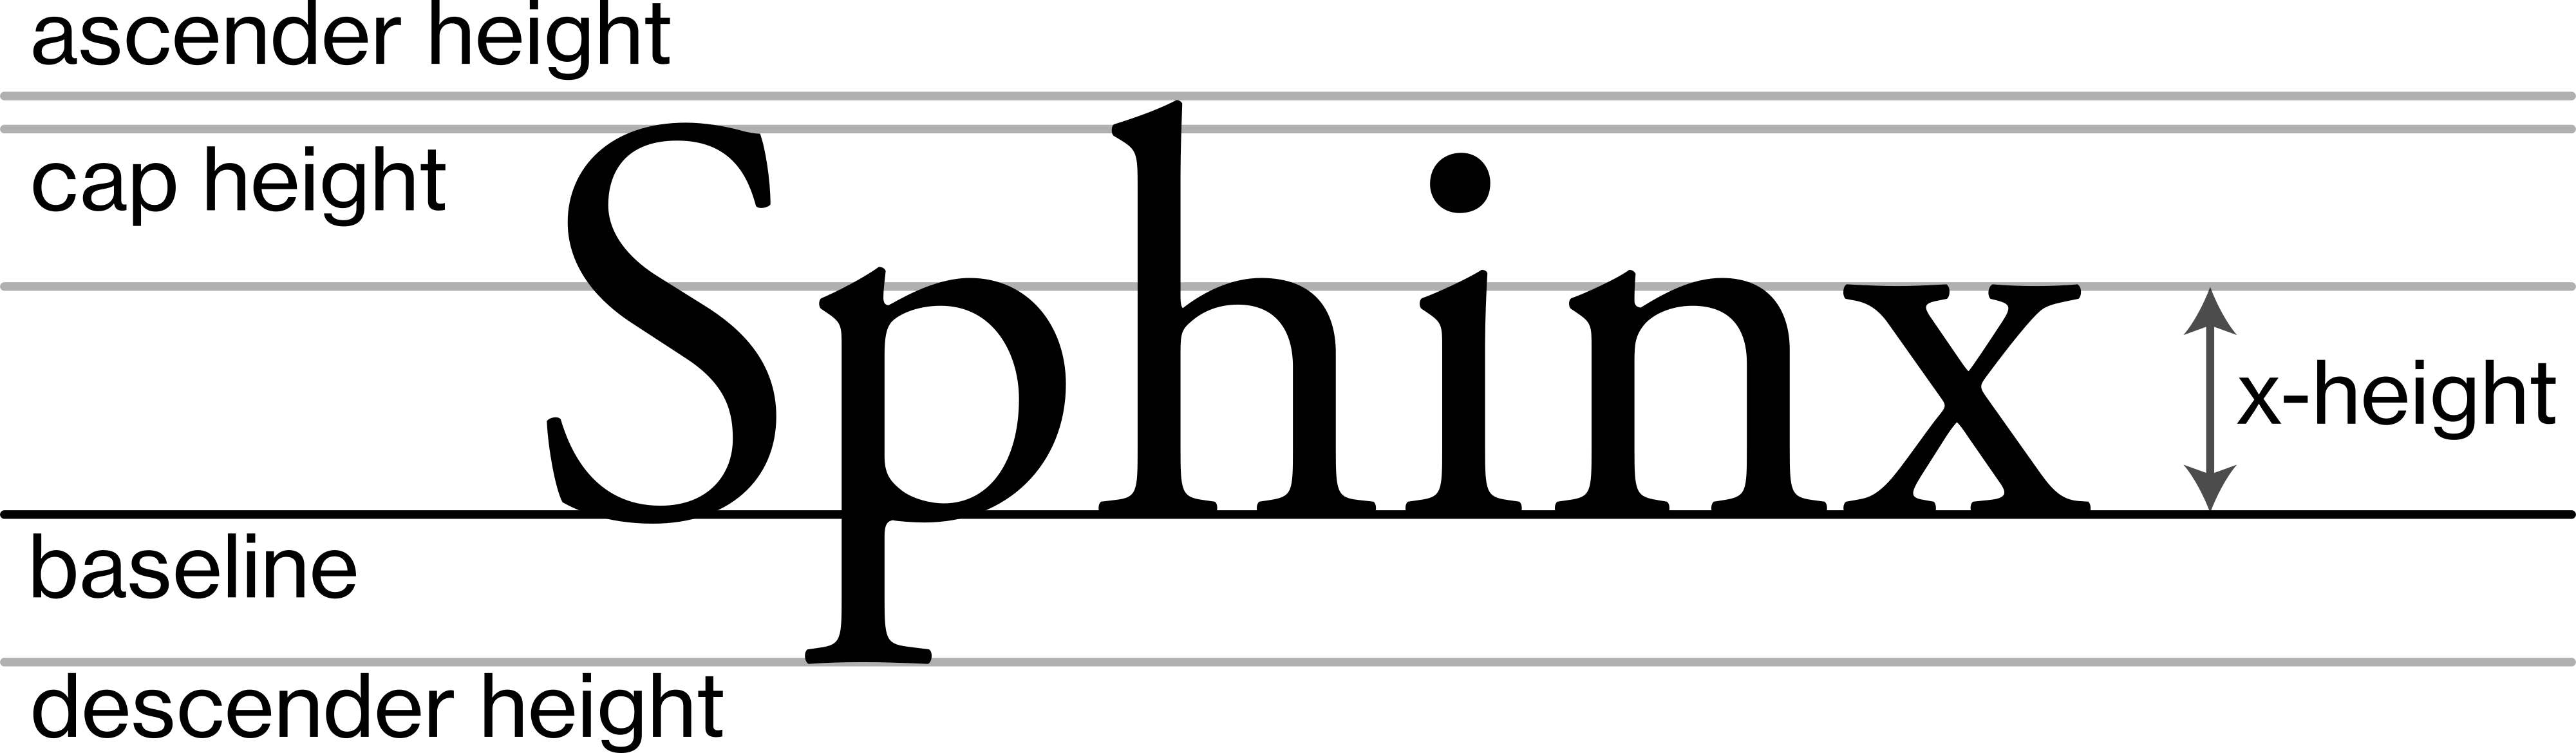
\includegraphics[keepaspectratio,width=0.65\textwidth]{heights.png}

\captionof{figure}{Common font metrics used in typography.
Text sits on the \introduce{baseline},
extends to the \introduce{ascender height},
and descends to the \introduce{descender height}.
The \introduce{cap height} refers to the size of uppercase letters,
and the \introduce{x-height} refers to the size of lowercase letters.
These values are different for each typeface,
and two set at the same point size might have very different heights.
Compare Helvetica to {\rmfamily Garamond}---the former has a much larger x-height.}

% For size reference:
%{\sffamily\fontsize{8pt}{8pt}\selectfont This is 8-point text.}
\vspace*{0.3\baselineskip minus 0.1\baselineskip}
\end{adjustwidth}

TODO: Talk about arbitrary sizes and leading.


\chapter{Punctuation}
\label{punctuation}

You would much rather encounter a panda that eats
shoots and leaves than one that eats, shoots,
and leaves.\punckern\endnote{Lynne Truss,
\textit{Eats, Shoots \& Leaves} (New York, 2003)}
Punctuation is a vital part of writing,
and there's more to it than your keyboard suggests.

\section{Quotation marks}

\LaTeX{} doesn't automatically convert ``straight'' quotes
into correctly-facing ``curly'' ones:
\begin{leftfigure}
\begin{lstlisting}
"This isn't right."
\end{lstlisting}
\end{leftfigure}
will get you
\begin{leftfigure}
\lm%
"This isn't right."
\end{leftfigure}
Instead, use \texttt{`} for opening quotes and \texttt{'} for closing
quotes.\punckern\footnote{Don't use \texttt{"} for closing double quotes.
Not only does \texttt{``example"} look a bit unbalanced,
but \texttt{"} is used as a formatting command when typesetting certain
languages, like German. (See \chapref{i18n} for more on international
typesetting.)}
\begin{leftfigure}
\begin{lstlisting}
``It depends on what the meaning of the word `is' is.''
\end{lstlisting}
\end{leftfigure}
quotes a former \acronym{us} president as,
\begin{leftfigure}
\lm%
``It depends on what the meaning of the word `is' is.''
\end{leftfigure}

\section{Hyphens and dashes}

Though they look similar,
hyphens (\,-\,), en dashes (\,--\,),
em dashes (\,---\,), and minus signs (\,$-$\,)
serve different purposes:
\begin{description}
\item[Hyphens] have a few uses:\endnote{Matthew Butterick,
    ``Hyphens and dashes''\quotekern,
    \textit{Practical Typography},
    \https{practicaltypography.com/hyphens-and-dashes.html}}
    \begin{itemize}[leftmargin=*]
    \item They allow a word to be split between the end of one line and the
        start of the next.
        \LaTeX{} usually handles this automatically.
    \item Some compound words use hyphens, like \emph{long-range}
        and \emph{field-effect}.
    \item They are used in phrasal adjectives.
        If I ask for ``five dollar bills''\punckern,
        do I want five \$1 bills, or several \$5 bills?
        It's clearer that I mean the latter when set as
        \emph{five-dollar bills}.
    \end{itemize}
    In \LaTeX{}, they are produced with the hyphen key (\,\texttt{-}\,).

\item[En dashes] indicate ranges such as ``pages 4--12''\quotekern,
    or separations like the ``US--Canada border''\quotekern.
    They are set with two adjacent hyphens (\,\texttt{--}\,).

\item[Em dashes] can be used to separate clauses of a sentence.
    Other punctuation marks---like parenthesis or commas---play a similar
    role.
    They are set with three adjacent hyphens (\,\texttt{---}\,).

\item[Minus signs] are used exclusively for negative quantities and
    mathematical expressions.
    They are often similar in length to an en dash,
    but sit at a different height.
    They are set with the hyphen key when in a math environment
    (see \chapref{math}), or with \verb|\textminus|.
\end{description}

\section{Ellipses}

A set of three dots used to indicate a pause or omission is called an
\introduce{ellipsis}.
It is set using \verb|\ldots|.
\begin{leftfigure}
\begin{lstlisting}
I'm\ldots{} not sure.
\end{lstlisting}
\end{leftfigure}
becomes
\begin{leftfigure}
\lm%
I'm\ldots{} not sure.
\end{leftfigure}

\section{Spacing}

As we discovered in our first example,
\LaTeX{} automatically inserts extra space between periods and whatever
follows them---presumably the start of the next sentence.
Sometimes, this isn't what we want!
Consider honorifics like Mr.\ and Ms., for example.
In situations like these, we also need to prevent \LaTeX{} from starting a
new line after the period.
This calls for a \introduce{non-breaking space}, which we set with a tilde.
\begin{leftfigure}
\begin{lstlisting}
Please call Ms.~Shrdlu.
\end{lstlisting}
\end{leftfigure}
produces proper spacing:
\begin{leftfigure}
\lm%
Please call Ms.~Shrdlu.
\end{leftfigure}

In other occasions, such as when we abbreviate units of
measurement,\punckern\footnote{There are also dedicated packages for doing so,
like \texttt{siunitx}.}
we want spaces that are thinner than usual inter-word ones.
For these, we use \verb|\,|\,:
\begin{leftfigure}
\begin{lstlisting}
Launch in 2\,h 10\,m.
\end{lstlisting}
\end{leftfigure}
announces
\begin{leftfigure}
\lm%
Launch in 2\,h 10\,m.
\end{leftfigure}

\section{What next?}
\begin{itemize}
\item Add hyphenations for uncommon words using \verb|\hyphenate|
    or \verb|\-|.\punckern\footnote{\LaTeX{} usually does a good
    job of automatically hyphenating words, based on a dictionary of patterns
    stored for each language. You should rarely need these tools.}
\item Learn other commands for spacing, such as \verb|\:|, \verb|\;|,
    \verb|\enspace|, and \verb|\quad|.
\item Use the \texttt{csquotes} package's \verb|\enquote| to simplify
    nested quotations, e.g., \\
    \enquote{She exclaimed, \enquote{I can't believe it!}}
\item Discover the typographical origins of terms like \introduce{en},
    \introduce{em}, and \introduce{quad}.
\item Familiarize yourself with the difference between \texttt{/} and
    \verb|\slash|.
\end{itemize}


\chapter{Layout}

\section{Justification and alignment}

\LaTeX{} is extraordinarily good at justifying text.
Instead of considering each line individually---as most word processors and
web browsers do---it examines all possible line breaks for a given paragraph,
then chooses ones that will give the best overall
spacing.\punckern\endnote{Donald E.~Knuth and Michael F.~Plass,
\textit{Breaking Paragraphs Into Lines} (Stanford, 1981)}
Combined with its ability to automatically hyphenate words,
which allows line breaks in many more places,\punckern\endnote{%
Franklin Mark Liang,
\textit{Word Hy-phen-a-tion by Com-put-er} (Standford, 1983),
\url{http://www.tug.org/docs/liang/}}
this produces some of the best paragraph layout available.

Sometimes we don't want to justify our text, though.
If you would prefer it be ``flush left''\quotekern,
with a ragged right side, place it in a \texttt{flushleft} environment,
or add \verb|\raggedright| to the current group.
To center it, place it in a
\texttt{center} environment, or add \verb|\centering| to the current group.
And to flush it against the right margin,
use a \texttt{flushright} environment or \verb|\raggedleft|.

\begin{leftfigure}
\begin{lstlisting}
\begin{flushleft}
This text is flush left with a ragged right edge.
Some prefer this layout since inter-word spacing
is more consistent than it is in justified text.
\end{flushleft}

\begin{center}
This text is centered.
\end{center}

\begin{flushright}
And this text is flush right.
\end{flushright}
\end{lstlisting}
\end{leftfigure}
sets
\begin{leftfigure}
\fbox{%
\begin{minipage}{0.7\textwidth}
\lm%
\begin{flushleft}
This text is flush left with a ragged right edge.
Some prefer this layout since inter-word spacing
is more consistent than it is in justified text.
\end{flushleft}

\begin{center}
This text is centered.
\end{center}

\begin{flushright}
And this text is flush right.
\end{flushright}
\end{minipage}
}
\end{leftfigure}

\section{Lists}

\LaTeX{} provides three environments for lists:
\texttt{itemize}, \texttt{enumerate}, and \texttt{description}.
In all three, each item starts with an \verb|\item| command.
The \texttt{itemize} environment uses bullets.
With:
\begin{leftfigure}
\begin{lstlisting}
\begin{itemize}
\item 5.56 millimeter
\item 9 millimeter
\item 7.62 millimeter
\end{itemize}
\end{lstlisting}
\end{leftfigure}
you get
\begin{leftfigure}
\lm%
\begin{itemize}[leftmargin=*]
\item 5.56 millimeter
\item 9 millimeter
\item 7.62 millimeter
\end{itemize}
\end{leftfigure}

\bigskip
\noindent The \texttt{enumerate} environment numbers your list:
\begin{leftfigure}
\begin{lstlisting}
\begin{enumerate}
\item Collect underpants
\item ?
\item Profit
\end{enumerate}
\end{lstlisting}
\end{leftfigure}
produces
\begin{leftfigure}
\lm%
\begin{enumerate}[leftmargin=*]
\item Collect underpants
\item ?
\item Profit
\end{enumerate}
\end{leftfigure}

\bigskip
\noindent The \texttt{description} environment starts each item with some
emphasized text, or \introduce{label}:
\begin{leftfigure}
\begin{lstlisting}
\begin{description}
\item[Alan Turing] was a British mathematician who laid much
    of the groundwork for the field of computer science.
    He is perhaps most remembered for his model of
    general-purpose computing, the Turing machine.
\item[Edsger Dijkstra] was a Dutch computer scientist.
    His contributions in many subdomains---such as concurrency
    and graph theory---are still in wide use today.
\item[Leslie Lamport] is an American computer scientist.
    He defined the concept of sequential consistency,
    which is used to safely communicate between tasks
    running in parallel on multiple processors.
\end{description}
\end{lstlisting}
\end{leftfigure}
gives us
\begin{leftfigure}
\begin{minipage}{0.8\textwidth}
\lm%
\begin{description}[leftmargin=*]
\item[Alan Turing] was a British mathematician who laid much
    of the groundwork for the field of computer science.
    He is perhaps most remembered for his model of
    general-purpose computing, the Turing machine.
\item[Edsger Dijkstra] was a Dutch computer scientist.
    His contributions in many subdomains---such as concurrency
    and graph theory---are still in wide use today.
\item[Leslie Lamport] is an American computer scientist.
    He defined the concept of sequential consistency,
    which is used to safely communicate between tasks
    running in parallel on multiple processors.
\end{description}
\end{minipage}
\end{leftfigure}

\section{Columns}

We often split documents---or parts of them---into multiple columns.
This is especially common when printing on \textsc{a4} or \acronym{us} letter
paper, since it allows a much more comfortable line widths at standard
8--12\,pt text sizes.\punckern\footnote{You'll see different advice depending
on where you look, but a general rule of thumb is to choose layouts that give
fewer than 90 characters per line (including spaces).
Shorter lines keep readers from having to scan very far to begin the next line,
which produces a more comfortable experience.}
You can either add the \texttt{twocolumn} option to your document class,
which splits everything into two columns, or you can use the \texttt{multicols}
environment from the \texttt{multicol} package:
\begin{leftfigure}
\begin{lstlisting}
One nice feature of \texttt{multicol} is that you can
combine arbitrary layouts.
\begin{multicols}{2}
In this example we start with one column,
then create a short section with two.
The package will ensure that the text inside is split
so each column is about the same height.
\end{multicols}
\end{lstlisting}
\end{leftfigure}
is split into
\begin{leftfigure}
\lm%
One nice feature of \texttt{multicol} is that you can
combine arbitrary layouts.
\begin{multicols}{2}
In this example we start with one column,
then create a short section with two.
The package will ensure that the text inside is split
so each column is about the same height.
\end{multicols}
\end{leftfigure}

\section{Page breaks}

Some commands, like \verb|\chapter| in a book, add their own page breaks.
You can insert your own with \verb|\clearpage|.
If you are using the \texttt{twoside} document class option for double-sided
printing, you can break to to the front of the next page with
\verb|\cleardoublepage|

\section{Footnotes}

Footnotes are a great tool for comments and asides which readers might
find useful, but aren't crucial to the main text.
Using the \verb|\footnote| command will cause the argument to be placed
in a footnote at the bottom of the current page:
\begin{leftfigure}
\begin{lstlisting}
I love footnotes!\footnote{Perhaps a bit too much\ldots}
\end{lstlisting}
\end{leftfigure}

\section{What next?}
\begin{itemize}
\item Control paragraph spacing, either using the relevant
KOMA~Script options, or with the \texttt{parskip} package.
\item Set the page size and margins with the \texttt{geometry} package.
\item Customize list formatting with the \texttt{enumitem} package.
\item Choose footnote symbols and layout with KOMA~Script and the
    \texttt{footmisc} package.
\item Insert horizontal and vertical space with commands like
    \verb|\vspace|, \verb|\hspace|, \verb|\vfill|, and \verb|\hfill|.
\item Learn what units \LaTeX{} provides for specifying spacing.
    (We've already mentioned a few here, such as
    \texttt{pt}, \texttt{bp}, \texttt{mm}, and \texttt{in}.)
\end{itemize}


\chapter{Mathematics}

\LaTeX{} is excellent at typesetting mathematics, both inline with body text,
e.g., $x_n^2+y_n^2=r^2$, and as standalone formulas:
\[\sum_{n=0}^{\infty} \frac{f^{(n)} (a)}{n!} (x - a)^n\]
The former is created with \verb|$...$| or \verb|\(...\)|,
and the latter with \verb|\[...\]|.
Inside these environments, the rules of \LaTeX{} change:
\begin{itemize}
\item Most spaces and line breaks are ignored completely,
    and the engine usually makes spacing decisions for you based on
    typographical conventions for math.
    \verb|$x+y+z$| and \verb|$x + y + z$| both give you $x+y+z$.
\item Empty lines are not allowed---each formula must occupy a single
    ``paragraph''\quotekern.
\item Letters are automatically italicized, as they are assumed to be variables.
\end{itemize}
To return to normal ``text mode'' inside a formula, use the \verb|\text| command.
Other formatting commands mentioned in \chapref{formatting} work as well.
From
\begin{leftfigure}
\begin{lstlisting}
\[\text{fake formulas} = \textbf{annoyed mathematicians}\]
\end{lstlisting}
\end{leftfigure}
we get
\[\text{\lm fake formulas} = \textbf{\lm annoyed mathematicians}\]

\section{Examples}

Typesetting mathematics is arguably the raison d'être of
\LaTeX,\punckern\footnote{Well, \TeX} but the topic is so broad that giving
it decent coverage would take up half the book.
Given how wide the field of mathematics is,
there are \emph{many} different commands and environments.
Here, more so than anywhere else,
you owe it to yourself to find some real references and learn what the system
is capable of.
Before moving on, though, let's show some examples of what \LaTeX{}
can do.
\newpage

\begin{enumerate}
\item \verb|x = \frac{-b \pm \sqrt{b^2 - 4 a c}}{2a}|
    \[x = \frac{-b \pm \sqrt{b^2 - 4 a c}}{2a} \]

\item \verb|e^{j \theta} = \cos(\theta) + j \sin(\theta)|
    \[e^{j \theta} = \cos(\theta) + j \sin(\theta)\]

\item
\begin{verbatim}
\begin{bmatrix}
x' \\
y'
\end{bmatrix} =
\begin{bmatrix}
\cos \theta &  -\sin\theta \\
\sin \theta & \cos \theta
\end{bmatrix}
\begin{bmatrix}
x \\
y
\end{bmatrix}
\end{verbatim}
\[
\begin{bmatrix}
x' \\
y'
\end{bmatrix} =
\begin{bmatrix}
\cos \theta &  -\sin\theta \\
\sin \theta & \cos \theta
\end{bmatrix}
\begin{bmatrix}
x \\
y
\end{bmatrix}
\]

\item
\begin{verbatim}
\oint_{\partial \Sigma} \mathbf{E} \cdot \mathrm{d}\boldsymbol{\ell}
    = - \frac{\mathrm{d}}{\mathrm{d}t}
      \iint_{\Sigma} \mathbf{B} \cdot \mathrm{d}\mathbf{S}
\end{verbatim}
    \[\oint_{\partial \Sigma} \mathbf{E} \cdot \mathrm{d}\boldsymbol{\ell}  = - \frac{\mathrm{d}}{\mathrm{d}t} \iint_{\Sigma} \mathbf{B} \cdot \mathrm{d}\mathbf{S}\]
\end{enumerate}


\chapter{Fonts}
\label{fonts}

Digital fonts have changed almost entirely in the past thirty years.
Originally, \LaTeX{} used \MF,
a system designed by Donald Knuth specifically for \TeX{}.
As time went on, support for PostScript\footnote{One of
Adobe's original claims to fame,
PostScript is a language for defining and drawing computer graphics,
including type. It remains in use today.} fonts was added.
Today, \LuaLaTeX{} and \XeLaTeX{} support the formats you're
most likely to encounter on your computer:
TrueType and OpenType.\punckern\footnote{Mac versions of \LaTeX{} also support
Apple's \acronym{aat}, but let's limit this discussion to
more ubiquitous formats.}

\begin{description}
\item[TrueType] was developed by Apple and Microsoft in the late 1980s.
    Most of the fonts that come pre-installed on your system are likely
    in this format.
    TrueType files generally end in a \monobox{.ttf} extension.
\item[OpenType] was first released in 1996 by Microsoft and Adobe.
    One major improvement over TrueType is its ability to embed
    various ``features''\quotekern, such as alternative glyphs
    and spacing options, in a single font file.
    OpenType files generally end in an \monobox{.otf} extension.
\end{description}

\section{Changing fonts}

By default, \LuaLaTeX{} and \XeLaTeX{} use Latin Modern,
an OpenType rendition of \LaTeX's original type family, Computer Modern.
While these are high-quality fonts,
they're probably not the only ones you ever want to use.
For others, we turn to the \texttt{fontspec} package:
\begin{leftfigure}
\begin{lstlisting}
\documentclass{article}

\usepackage{fontspec}
\setmainfont[Ligatures=TeX]{Source Serif Pro}
\setsansfont[Ligatures=TeX]{Source Sans Pro}
\setmonofont{Source Code Pro}

\begin{document}
Hello, Source type family! Neat---no? \\
\sffamily Let's try sans serif! \\
\ttfamily Let's try monospaced!
\end{document}
\end{lstlisting}
\end{leftfigure}
should produce something like\footnote{Assuming, of course,
that you have Adobe's open-source fonts installed.\punckern\endnote{Adobe's
open-source typefaces are freely available at
\https{github.com/adobe-fonts}}}
\begin{leftfigure}
\fontspec[Ligatures=TeX]{Source Serif Pro} Hello, Source type family! Neat---no? \\
\fontspec[Ligatures=TeX]{Source Sans Pro} Let's try sans serif! \\
\fontspec{Source Code Pro} Let's try monospaced!
\end{leftfigure}
The \verb|Ligatures=TeX| option enables the standard punctuation
shortcuts discussed in \chapref{punctuation} (e.g., creating en dashes with
\texttt{--} or curly quotes with \texttt{``}) instead of forcing you
to type the the corresponding characters, which probably aren't on your keyboard.
You often don't want these for monospaced type, though,
since the text you set in it---such as code---is meant to be displayed
verbatim. \verb|"Hello!"| shouldn't turn into
\verb|“Hello!“|.

\section{Selecting font files}

Typefaces come packaged as multiple files for their various
weights and styles---a typical set includes upright,
\textit{italics},
\textbf{bold}, and
\textit{\textbf{bold italics}}.
\texttt{fontspec} can generally deduce the appropriate file
names given the name of the typeface.\punckern\footnote{This is
one of the places \XeLaTeX{} and \LuaLaTeX{}
differ in a way that's noticeable to the casual user.
The former generally uses system libraries---such as FontConfig on Linux---to
locate files from a typeface's name.
The latter has its own font loader,
based on code from FontForge.\punckern\endnote{\textit{\LuaTeX{} Reference}
(Version 1.0.4, February 2017), 10}
The expected name of a font might differ between the two engines---refer
to the \texttt{fontspec} manual for details.}
However, many typefaces come in more than two weights---some versions of Futura,
for example, come in
{\fontspec[Scale=MatchLowercase]{Futura-Lig}light},
{\fontspec[Scale=MatchLowercase]{Futura-Boo}book},
{\fontspec[Scale=MatchLowercase]{Futura-Med}medium},
{\fontspec[Scale=MatchLowercase]{Futura-Dem}demi},
{\fontspec[Scale=MatchLowercase]{Futura-Bol}bold}, and
{\fontspec[Scale=MatchLowercase]{Futura-ExtBol}extra bold}.
Sometimes
{\fontspec[Scale=MatchLowercase]{FuturaSc-Boo}\textsc{small caps}}
are stored in separate files as well.\punckern\footnote{OpenType allows
small caps to be placed in the same file(s) as the other glyphs.
If your font supports this, you don't need to do anything---\texttt{fontspec}
will dutifully switch to them whenever you use
\monobox{\textbackslash textsc} or \monobox{\textbackslash scshape}.
But for TrueType, and for OpenType fonts that don't take advantage of this
feature, you'll have to load a separate file as shown here.}

We might want to hand-pick weights to achieve a certain look or better match the
weights of other fonts in our document.\punckern\footnote{Compare how
{\fontspec[Scale=MatchLowercase]{Futura-Lig}the light,}
{\fontspec[Scale=MatchLowercase]{Futura-Boo}book,}
{\fontspec[Scale=MatchLowercase]{Futura-Med}and medium weights}
of Futura look compared to surrounding type on this page.}
Continuing to use Futura as an example,
say we want to use the ``book'' weight as our default
and ``demi'' for bold.
Assuming the font files are named:
\begin{itemize}
\item \monobox{Futura-Boo} for our
    {\fontspec[Scale=MatchLowercase]{Futura-Boo}upright book weight}
\item \monobox{Futura-BooObl} for our
    {\fontspec[Scale=MatchLowercase]{Futura-BooObl}oblique book weight}
\item \monobox{FuturaSC-Boo} for
    {\fontspec[Scale=MatchLowercase]{FuturaSC-Boo}small caps, book weight}
\item \monobox{Futura-Dem} for
    {\fontspec[Scale=MatchLowercase]{Futura-Dem}upright demi(bold)}
\item \monobox{Futura-DemObl} for
    {\fontspec[Scale=MatchLowercase]{Futura-DemObl}oblique demibold}
\end{itemize}

\noindent Our setup might resemble:
\begin{leftfigure}
\begin{lstlisting}
\usepackage{fontspec}
\setmainfont[
    Ligatures=TeX,
    UprightFont = *-Boo,
    ItalicFont = *-BooObl,
    SmallCapsFont = *SC-Boo,
    BoldFont = *-Dem,
    BoldItalicFont = *-DemObl
]{Futura}
\end{lstlisting}
\end{leftfigure}
Note that instead of typing out \monobox{Futura-Boo},
\monobox{Futura-BooObl}, and so on, we can use \texttt{*} to insert the base name.

\section{Scaling}

Creating a cohesive look with multiple fonts is tricky,
especially since typefaces might look completely different
at the same point size.
\texttt{fontspec} can help a bit here by scaling fonts to match either the
x-height or the cap height of your main font with
\verb|Scale=MatchLowercase| or \verb|Scale=MatchUppercase|,
respectively.\footnote{One way to sidestep this issue is to have fewer
typefaces in your design. Even just one or two,
used carefully, can produce amazing results.}


\section{OpenType features}

As mentioned at the start of the chapter,
OpenType fonts provide various features that can be turned on and off.
In \LaTeX{}, these are controlled with optional arguments to
\verb|\setmainfont| and friends.
They can also be set for the current group with
\verb|\addfontfeature|.
Let's touch on a few common ones.

\subsection{Ligatures}

Many typefaces use \introduce{ligatures}, which combine multiple characters
into a single glyph.\punckern\footnote{Ligatures fell out
of style during the 20{\addfontfeature{VerticalPosition=Superior}th}
century due to limitations of printing technology and the increased popularity
of sans serif typefaces, which often lack them.
Today they are making a comeback,
thanks in no small part to their support in OpenType.}
OpenType groups ligatures into three categories:
\begin{description}
\item[Standard] ligatures are enabled by default, and remedy spacing problems
    a typeface might otherwise have. Consider the lowercase letters f
    and i.
    In many serif typefaces, these combine
    to form the ligature fi, which avoids awkward spacing between f's ascender
    and i's dot
    {\addfontfeature{Ligatures=CommonOff} (\,fi\,)}.
    Other common examples in English writing include ff,
    ffi, fl, and ffl.
\item[Discretionary] ligatures, such as
    {\addfontfeature{Ligatures=Discretionary}ct},
    are offered by some fonts.
    They are disabled by default
    but can be enabled with
    \verb|Ligatures=Discretionary|.
\item[Historical] ligatures are ones which have fallen out of common use,
    such as those with a \introduce{long~s} (e.g., ſt).
    These are also disabled by default
    but can be enabled with \verb|Ligatures=Historic|.
\end{description}
Multiple options can be grouped together.
Say you want discretionary ligatures.
In the likely event that you also want \verb|Ligatures=TeX|,
you would enable both with
\verb|Ligatures={TeX,Discretionary}|.
Ligatures can also be disabled with corresponding \verb|*Off|
options. If you want to stop using discretionary ligatures for some passage,
\begin{leftfigure}
\begin{lstlisting}
{\addfontfeature{Ligatures=DiscretionaryOff}...}
\end{lstlisting}
\end{leftfigure}
does the trick.

Some words are arguably typeset better without ligatures---a classic example
is shelfful.\punckern\endnote{Knuth, \textit{The \TeX book},
(Addison-Wesley, 1986), 19}
You can manually prevent the insertion of ligatures with a zero-width space,
e.g., \verb|shelf\hspace{0pt}ful|,
or use the \texttt{selnolig} package to handle most of these cases automatically.

\subsection{Figures}

When setting figures,\punckern\footnote{\introduce{Figure}
here refers to what some might call a \introduce{numeral} or
\introduce{digit}---i.e., 0, 1, 2, 3, 4, 5, 6, 7, 8, 9.
Typographers generally prefer the first term to the other two.}
you have two
choices to make: lining versus oldstyle,
and proportional versus tabular.
\introduce{Lining} figures, sometimes called \introduce{titling} figures,
have similar heights as capital letters:
\begin{leftfigure}
\addfontfeature{Numbers=LowercaseOff}
A B C D 1 2 3 4
\end{leftfigure}
\introduce{Oldstyle}, or \introduce{text} figures,
share more similarities with lowercase letters:
\begin{leftfigure}
Sitting cross-legged on the floor\ldots{} 25 or 6 to 4?
\end{leftfigure}
For body text, either choice is fine, but oldstyle figures shouldn't
be combined with capital letters.
``F-15C'' looks odd, as does ``V2.3 Release''\quotekern.

{\addfontfeature{Numbers=LowercaseOff}
The terms \introduce{proportional} and \introduce{tabular} refer to spacing.
Tabular figures are set with a uniform width, such that 1 takes up
the same space as 8.
As their name suggests, this is great for tables and other scenarios
where figures must line up in columns:}
\begin{leftfigure}
\addfontfeature{Numbers={Tabular,LowercaseOff}}
\begin{tabular}{l|c r}
Item & Qty. & Price \\
\hline
Gadgets & 42 & \$5.37 \\
Widgets & 18 & \$12.76 \\
\end{tabular}
\end{leftfigure}
Proportional figures are the opposite---their spacing is, well\ldots{}
\emph{proportional} to the width of the figure.
They are usually preferred in body text, where 1837
looks a bit nicer than
{\addfontfeature{Numbers=Tabular}1837}.

You select figures with the following options:
\begin{leftfigure}
\begin{tabular}{l l}
\texttt{Numbers=} & \texttt{Lining / Uppercase} \\
 & \texttt{OldStyle / Lowercase} \\
 & \texttt{Proportional} \\
 & \texttt{Tabular / Monospaced}
\end{tabular}
\end{leftfigure}
As with ligatures, traits can be combined:
you get proportional lining figures
with \texttt{Numbers=\allowbreak\{Proportional,\allowbreak Lining\}},
or tabular oldstyle figures with
\texttt{Numbers=\allowbreak\{Tabular,\allowbreak OldStyle\}}.
Each option also has a corresponding \verb|*Off|
variant.\punckern\footnote{This is especially useful since fonts
select figures in different ways.
In some, the default figures are lining
and oldstyle figures are enabled with
\monobox{Numbers=OldStyle}.
To return to lining figures,
\monobox{Numbers=Lining}
doesn't work, but
\monobox{Numbers=OldStyleOff}
does.}

Finally, some fonts provide \introduce{superior and inferior} figures,
which are useful for ordinals
(\otford{1}{st}, \otford{2}{nd} \otford{3}{rd}, \ldots),
fractions (\,\otffrac{25}{624}\,), and so on.
These have the same weight as their full-sized counterparts,
which looks much better than shrinking the font's normal figures.
(Compare the above to
{\fontspec[OpticalSize=0]{garamondpremrpro}%
\mbox{1\textsuperscript{st}},
\mbox{2\textsuperscript{nd}},
\mbox{3\textsuperscript{rd}},
and
\,\mbox{\textsuperscript{25}^^^^2044\textsubscript{624}}%
\,}.
Notice how this second set is too light compared to the surrounding
type.)
They are selected with:
\begin{leftfigure}
\begin{tabular}{l l}
\texttt{VerticalPosition=} & \texttt{Superior / Inferior}
\end{tabular}
\end{leftfigure}

\section{What next?}
\begin{itemize}
\item See how \texttt{fontspec} chooses fonts based on point size when multiple
    optical sizes are available, either automatically via OpenType,
    or manually using \texttt{SizeFeatures}.
\item Experiment with letter spacing---or \introduce{tracking}---with
    the \texttt{LetterSpace} option.
    Extra tracking is unnecessary in most cases,
    but can be useful to make \textsc{small caps}
    a bit more \acronym{readable}.
\end{itemize}


\chapter{Microtypography}
\label{microtype}

\introduce{Microtypography} is the craft of improving a document's legibility
with small, subliminal tweaks.
In other words, it is
\begin{quote}
[\dots]the art of enhancing the appearance and readability of a
document while exhibiting a minimum degree of visual obtrusion.
It is concerned with what happens between or at the margins of characters,
words or lines. Whereas the macro-typographical aspects of a document
(i.e., its layout) are clearly visible even to the untrained eye,
micro-typographical refinements should ideally not even be recognisable.
That is, you may think that a document looks beautiful, but you
might not be able to tell exactly why: good micro-typographic practice tries to
reduce all potential irritations that might disturb a reader.\punckern\endnote{%
R Schlicht,
\textit{The microtype package}
(v2.7a, January 14, 2018), 4}
\end{quote}

In \LaTeX{}, microtypography is controlled with the
\texttt{microtype} package.
Its use is automatic---for the vast majority of documents, you should add
\begin{leftfigure}
\begin{lstlisting}
\usepackage{microtype}
\end{lstlisting}
\end{leftfigure}
to your preamble and carry on---but let's take a brief look at what the package
does.

\section{Character protrusion}

By default, \LaTeX{} justifies lines between perfectly straight
left and right margins.
This is the obvious choice,
but falls victim to an annoying optical illusion:
lines ending in small glyphs---like periods, commas,
or hyphens---seem shorter than lines that
don't.\punckern\footnote{Many other optical illusions come up in typography.
For example, if a circle, a square, and a triangle
of equal heights are placed next to each other,
the circle and triangle look smaller than the square.
For this reason, round or pointed characters (like O and A) must
be made slightly taller than ``flat'' ones (such as H and T) for all
to appear the same height.\punckern\endnote{%
Jost Hochuli, \textit{Detail in typography}
(Éditions~\textsc{b}42, 2015),
18--19}}
\texttt{microtype} compensates by \introduce{protruding} these smaller glyphs
into the margins.

\section{Font expansion}

In order to to help \LaTeX's justification algorithm build paragraphs with
more even spacing and fewer hyphenated lines,
\texttt{microtype} can stretch characters horizontally.
You might think that distorting the type this way would be immediately
noticeable,
but you're reading a book that does so on every page!
This effect, called \introduce{font expansion},
is applied \emph{very} slightly---by default,
character widths are altered by no more than two percent.\punckern\footnote{%
Of course, you can use package options to change this limit,
or disable the feature entirely.}

This feature isn't currently available for \XeLaTeX{}.
You'll need to use \LuaLaTeX{} if you'd like to take advantage of it.

\section{What next?}

As always, see the package manual for ways to tweak these features.
\texttt{microtype} is capable of a few other tricks,
but several only work on older \LaTeX{} engines.\punckern\footnote{i.e., pdf\TeX}
Those we do care about---such as letterspacing---can be handled with
\texttt{fontspec} or other packages.


\chapter{Typographie Internationale}
\label{i18n}

Surprisingly, many languages besides English exist.
You may want to write with them.

\section{Unicode}

Digitising human language is a complicated topic that has evolved significantly
since \LaTeX's inception, but today,
computers usually represent text with Unicode. Briefly,
\begin{itemize}
\item A Unicode text file is made of a series of \introduce{code points},
    each of which can represent a character to be drawn,
    an accent or other diacritical mark to combine with an adjacent character,
    or some non-printing character,
    such as an instruction to print subsequent text right-to-left.
\item One or more of these code points combines to represent a
    \introduce{grapheme cluster} or \introduce{glyph},
    the shapes within a font that we informally call ``characters''\quotekern.
\begin{centerfigure}
\large%
\fontspec[Ligatures=TeX]{NotoSerif}%
Приве́т
\quad\fontspec[Ligatures=TeX]{NotoSerif-Devanagari}%
नमस्ते
\captionof{figure}{How many characters do you see?
How many code points are they built from?}
\end{centerfigure}
\item Modern font formats contain encoding tables
    which map code points to the glyphs the file contains.
\end{itemize}
\LuaLaTeX{} and \XeLaTeX{} use these tools to render documents
from Unicode input
files.\punckern\footnote{LuaLaTeX accepts \mbox{\acronym{utf}-8} files,
while \XeLaTeX{} is a bit more flexible and also
accepts \mbox{\acronym{utf}-16} and
\mbox{\acronym{utf}-32}.}
Make sure that the fonts you select contain the needed glyphs---many
only contain ones for Latin languages.

\section{The polyglossia package}

If your document contains anything besides English,
you should use the \texttt{polyglossia} package.
It will automatically:
\begin{itemize}
\item Load language-specific hyphenation patterns and other typographical
    conventions.
\item Switch between fonts for each language, as specified by the user.
\item Translate document labels,
    like ``chapter''\quotekern, ``section''\quotekern, and so on.
\item Format dates according to language-specific conventions.
\item Format numbers in languages that have their own numbering system.
\item Use the \texttt{bidi} package for documents with languages written
    right to left.
\item Set the script and language tags of the current font, if applicable.
\end{itemize}
When using the package, specify the main language of your document,
along with any other languages you use.
Some languages also take regional dialects as an optional argument:
\begin{leftfigure}
\begin{lstlisting}
\usepackage{polyglossia}
\setdefaultlanguage[variant=american]{english}
\setotherlanguage{french}
\end{lstlisting}
\end{leftfigure}
\texttt{polyglossia} will define an environment for each loaded language.
These automatically apply that language's conventions to the text within.
French, for example, places extra space around punctuation, so
\begin{leftfigure}
\begin{lstlisting}
Dexter cried,
\begin{french}
«Omelette du fromage!»
\end{french}
\end{lstlisting}
\end{leftfigure}
gives\footnote{Yes, it's \emph{omelette au fromage}.
Direct all complaints to Cartoon Network.}
\begin{leftfigure}
\lm%
Dexter cried,
\begin{french}
\lm%
«Omelette du fromage!»
\end{french}
\end{leftfigure}

% FFS: https://github.com/reutenauer/polyglossia/issues/68
\directlua{polyglossia.desactivate_frpt()}

\section{What next?}
\begin{itemize}
\item See the \texttt{polyglossia} manual for language-specific commands.
\item Look into the \texttt{babel} package as an alternative to
    \texttt{polyglossia}.\punckern\footnote{\texttt{polyglossia} has better
    support for OpenType font features via \texttt{fontspec}.
    However, it is newer and has a few known bugs.
    \texttt{babel} is a fine substitute if you run into trouble.}
    %as I did in
    %\LuaLaTeX{} (see \url{https://github.com/reutenauer/polyglossia/issues/68}),
\item Try typesetting Japanese or Chinese with the \texttt{xeCJK} or
    \monobox{luatex-ja} packages.
\end{itemize}


\chapter{When Good Typesetting Goes Bad}

With luck, you're off to a good start with \LaTeX.
But as with any complicated tool, you'll eventually run into trouble.
Here are some common problems and what you can try to fix them.

\section{Fixing overflow}

\mbox{When \LaTeX{} can't fit a line into a paragraph with good spacing,
it gives up, overflowing} the line into the margin.
You can sometimes remedy this with some ``emergency stretch''\quotekern.
When you add \texttt{\textbackslash emergencystretch=\allowbreak<width>}
to the document's preamble,
\LaTeX{} will try to set troublesome paragraphs a second time,
stretching or shrinking the space in each line by up to the provided
width.\punckern\footnote{\LaTeX{} has pretty sane default limits to how much
it stretches and shrinks spacing in a paragraph.
You probably don't want to make \texttt{<width>} larger than an em or two.}
If that still doesn't help, try tweaking the wording of guilty paragraphs.
This can be frustrating, but the alternative is for \LaTeX{} to create spacing
that is too loose---where\quad
words\quad have\quad large\quad gaps\quad between\quad
them---or too tight, where\! words\! are\! awkwardly\! crammed\! together.

\section{Avoiding widows and orphans}

Typesetters do their best to avoid \introduce{widow} lines,
which appear separated from the rest of their paragraph at the start of the
following page.
They also avoid \introduce{orphan}, or \introduce{club} lines,
which are ``left behind'' on the previous page while the rest of the paragraph
begins the next.
\LaTeX{} tries to avoid these, but unfortunately, its page-splitting algorithm
is much more simplistic than the one it uses
to split paragraphs into lines.\punckern\footnote{This is because
1980s computers didn't have enough \acronym{ram} to do so. Seriously---Knuth
wrote at the time,
``The computer doesn't have enough high-speed memory capacity to remember the
contents of several pages,
so \TeX{} simply chooses each page break as best it can, by a process of
`local' rather than `global' optimization.\quotekern''\,\endnote{Knuth,
\textit{The \TeX book}, 110}}
You can make \LaTeX{} try harder to avoid orphans and widows with:
\begin{leftfigure}
\begin{lstlisting}
\widowpenalty=<penalty>
\clubpenalty=<penalty>
\end{lstlisting}
\end{leftfigure}
\verb|<penalty>| is a value between 0 and 10000.
When these values are maximized,
\LaTeX{} is never allowed to leave orphans or widows,
at \emph{any} cost.\punckern\footnote{When considering a given layout,
\LaTeX{} assigns penalties, or ``badness''\quotekern,
to anything that arguably makes a document look worse.
It chooses whichever layout it can find with the least badness.}
This may cause odd layouts to be chosen,
so be sure to review your pages if you choose large penalties.

\section{Handling syntax errors}
If you confuse \LaTeX{}---say, by issuing commands that don't exist,
or forgetting to end an environment---it will print an
error message,\punckern\footnote{Usually this contains a succinct summary of
the problem and the number of the line(s) it occurred on. Occasionally,
\LaTeX{} gets \emph{really} confused and emits something so cryptic it gives
\cpp{} template errors a run for their money.
As you continue to use \LaTeX, you'll start to get a feel for what sorts of
mistakes cause these rare, but enigmatic messages.}
then display an interactive prompt starting with \texttt{?}\,.
Here you can enter instructions for how to proceed.
Once upon a time, when computers were thousands of times slower and
\LaTeX{} took that much longer to re-run, this was more useful.
Today, we probably just want to quit,
then try again once we've fixed our document.
To exit the prompt, type \texttt{X}, then press Enter.
Better yet, you can tell \LaTeX{} to give up as soon as it finds trouble
by running your engine with the \monobox{-halt-on-error} flag:
\begin{leftfigure}
\begin{lstlisting}
$ lualatex -halt-on-error myDocument.tex
\end{lstlisting}
\end{leftfigure}


\appendix

\chapter{A Brief History of \texorpdfstring{\LaTeX}{LaTeX}}

\label{history}

Donald Knuth is celebrated among programmers as
the man who coined the term \emph{analysis of algorithms}
and pioneered many computer science fundamentals we use today.
Knuth is perhaps most famous for his ongoing magnum opus,
\textit{The~Art of Computer Programming}.

When the first volume of \acronym{taocp} was released in 1968,
it was printed the same way most books had been since the turn of the century:
with \introduce{hot metal} type.
Letters were cast from molten lead,
then arranged into lines.
These lines were clamped together to form pages,
which were inked and pressed against paper.

By March of 1977, Knuth was ready for a second run of \acronym{taocp}, volume~2,
but he was horrified when he received the proofs.
Hot metal typesetting was expensive, complicated, and time-consuming,
so publishers had replaced it with phototypesetting,
which works by projecting images of characters onto film.
The new technology, while much cheaper and faster,
didn't provide the quality Knuth
expected.\punckern\endnote{Knuth, \textit{Digital Typography} (Stanford, 1999), 3--5}

The average author would have resigned themselves to this change and moved on,
but Knuth took great pride in his books' appearances,
especially for their mathematics.
Around this time, he also discovered the growing field of digital typesetting,
where glyphs are built from tiny dots,
packed together at over 1,000 per inch.
Inspired,
Knuth set off on one of the greatest yak shaves\footnote{Programmers
call seemingly unrelated work needed to solve their main problem
``yak shaving''\quotekern. The phrase is thought to originate from an episode
of \textit{The Ren~\&~Stimpy Show}.\punckern\endnote{``yak shaving''\quotekern,
\textit{The Jargon File},
\href{http://www.catb.org/~esr/jargon/html/Y/yak-shaving.html}%
{\texttt{www.catb.org/\~{}esr/jargon/html/Y/yak-shaving.html}}}}
of all time.
For years, he paused work on his books to create his own
typesetting system.
When the dust settled in 1978, Knuth had the first version of
\TeX.\punckern\footnote{The name ``\TeX{}'' comes from the Greek
{\fontspec[Scale=MatchLowercase]{NotoSerif-Medium}τέχνη},
meaning \introduce{art} or \introduce{craft}.\punckern\endnote{Knuth,
\textit{The \TeX book}, 1}}

It's hard to appreciate how much of a revolution \TeX{} was,
especially looking back from a time where anybody with a copy
of Word can be their own desktop publisher.
Adobe's \acronym{pdf} wouldn't exist for another decade, so Knuth
and his graduate students devised their own device-independent format,
\acronym{dvi}.
Scalable fonts were uncommon, so he created \MF{} to rasterize glyphs
into dots on the page.
Perhaps most importantly, Knuth and his students designed algorithms
to automatically hyphenate and justify text into
beautifully-typeset paragraphs.\punckern\footnote{These same algorithms went
on to influence the ones Adobe uses in its software today.\punckern\endnote{%
Several sources (\http{www.tug.org/whatis.html},
\https{tug.org/interviews/thanh.html},
\http{www.typophile.com/node/34620})
mention \TeX's influence on the \textit{hz}-program by Peter Karow
and Hermann Zapf, thanks to via Knuth's collaborations with Zapf.
\textit{hz} was later acquired by Adobe and used
when creating InDesign's paragraph formatting systems.}}

\LaTeX{}, short for Lamport~\TeX{}, was later developed by Leslie Lamport
as a set of commands for common document layouts.
It was introduced in 1986 with his guide,
\textit{\LaTeX: A~Document Preparation System}.
Other typesetting systems based on \TeX{} also exist,
the other most popular today being Con\TeX{}t.

Development continues,
both in the form of user-provided packages for \TeX{} and \LaTeX{},
and as improvements to the \TeX{} typesetting program itself.
There are four versions, or \introduce{engines}:
\begin{description}
\item[\TeX] is the original system by Donald Knuth.
Knuth stopped adding features after version 3.0 in March~1990,
and all subsequent releases have contained only bug fixes.
With each release, the version number asymptotically approaches $\pi$
by adding an additional digit.
The most recent version, 3.14159265, came out in January~2014.

\item[pdf\TeX] is an extension of \TeX{} that provides direct \acronym{pdf}
    output (instead of \TeX's \acronym{dvi}),
    native support for PostScript
    and TrueType fonts,
    and micro-typographic features discussed in \chapref{microtype}.
    It was originally developed by
    Hàn Thế Thành
    as part of his PhD thesis
    for Masaryk University in Brno, Czech Republic.\punckern\endnote{%
    Hàn Thế Thành,
    \textit{Micro-typographic extensions to the \TeX{} typesetting system}
    (Masaryk University Brno, October 2000)}

\item[\XeTeX] is a further extension of \TeX{} that adds native support for
    Unicode and OpenType.
    It was originally developed by Jonathan Kew in the early 2000s,
    and gained full cross-platform support in 2007.\punckern\endnote{Jonathan Kew,
    ``\XeTeX{} Live''\quotekern, \textit{TUGboat} 29, no.~1 (2007)}

\item[\LuaTeX] is similar to \XeTeX{} in its native Unicode and modern font support.
    It also embeds the Lua scripting language into the engine,
    exposing an interface for package and document authors.
    It first appeared in 2007 and is developed by a core team of
    Hans Hagen, Hartmut Henkel, Taco Hoekwater,
    and Luigi Scarso.\punckern\endnote{\http{www.luatex.org}}
\end{description}

Building \TeX{} today is an\dots{} interesting endeavor.
When it was written in the late 1970s,
there were no large, well-documented open-source projects for students to study,
so Knuth set out to make \TeX{} into one.
As part of this effort, \TeX{} was written in a style he calls
\introduce{literate programming}: opposite most programs---where
documentation is interspersed throughout the code---Knuth wrote \TeX{} as a book,
with the code interspersed between paragraphs.
This mix of English and code is called \texttt{WEB}.\punckern\footnote{Knuth
also released a pair of companion programs named
\texttt{TANGLE} and \texttt{WEAVE}.
The former extracts the book---as \TeX, of course---and the latter
produces \TeX's Pascal source code.}

Unsurprisingly, most modern systems don't have good tooling for the late 1970s
dialect of Pascal that \TeX{} was written in,
so present-day distributions use another program,
\texttt{web2c}, to convert its \texttt{WEB} source into C code.
pdf\TeX{} and \XeTeX{} are built by combining the result with other C
and \cpp{} sources.
Instead of following this complicated process,
the \LuaTeX{} authors hand-translated Knuth's Pascal into C.
They have used the resulting code since 2009.\punckern\endnote{%
Taco Hoekwater, \textit{\LuaTeX{} says goodbye to Pascal}
(MAPS 39, Euro\TeX{} 2009),
\https{www.tug.org/TUGboat/tb30-3/tb96hoekwater-pascal.pdf}}



\setlength\parskip{0.8\baselineskip}
\setlength\parindent{0pt}

\chapter{Additional Resources}
\label{resources}

\section{For \texorpdfstring{\LaTeX}{LaTeX}}

As promised at the start, this book is incomplete.
To keep things short,
major \LaTeX{} features---like figures, captions, and graphics---haven't
been discussed.
Use some of these resources to fill in the gaps:

\begin{adjustwidth}{1.5em}{0pt}
The \LaTeX{} Wikibook, at \url{https://en.wikibooks.org/wiki/LaTeX}

The \TeX{} Stack Exchange, at \url{https://tex.stackexchange.com/}

\textit{The Not So Short Introduction to \LaTeX}, \\
available at \url{https://www.ctan.org/tex-archive/info/lshort/english/}

The Share\LaTeX{} knowledge base, at \url{https://www.sharelatex.com/learn}

\end{adjustwidth}

\section{For typography}

We've spent most of our time here focusing \emph{what} you can do with \LaTeX,
and little on \emph{how} you should use it to create well-designed documents.
Read on:

\begin{adjustwidth}{1.5em}{0pt}
\textit{Practical Typography}, by Matthew Butterick. \\
Available (for free!) at \url{https://practicaltypography.com}

\textit{Stop Stealing Sheep \& Find Out How Type Works}, by Erik Spiekermann

\textit{Thinking With Type}, by Ellen Lupton

\textit{The Elements of Typographic Style}, by Robert Bringhurst

\textit{Detail in Typography}, by Jost Hochuli
\end{adjustwidth}

\backmatter

\setkomafont{chapter}{\Huge\itshape}

{\raggedright
\renewcommand\makeenmark{\theenmark.\enspace}
% Chicago Manual of Style, Notes & Bib style, ish.
% http://www.chicagomanualofstyle.org/tools_citationguide/citation-guide-1.html
\theendnotes
}

% Redefine cleardoublepage so the Colophon doesn't demand a front page.
% From https://tex.stackexchange.com/a/24068/92465
{\let\cleardoublepage\clearpage \chapter{Colophon}}

This guide was typeset with \LuaLaTeX{} in Garamond Premier by Robert Slimbach.
His revival is based on roman type by
\otford{16}{th} century French
punchcutter Claude Garamond.
Italics are inspired by the work of Garamond's contemporary Robert Granjon.

Monospaced items are set in Matthias Tellen's
\href{https://madmalik.github.io/mononoki/}{\texttt{mononoki}},
a typeface designed to work well on both low-resolution computer monitors
and in high-resolution print.

Captions are set in
\href{http://www.fontbureau.com/NHG/}{\textsf{\small Neue Haas Grotesk}},
a Helvetica restoration by Christian Schwartz.
Other digitizations of the classic Swiss typeface are based on fonts made for
Linotype and phototypesetting machines,
resulting in digital versions with all the compromises and kludges from those
past two generations of printing technology.
Schwartz based his work on Helvetica's original drawings,
producing a design faithful to the original cold metal type.

{\fontspec[Ligatures=TeX, Scale=MatchLowercase]{Futura-Boo}URW Futura}
makes a few guest appearances.
Originally released in 1927 by Paul Renner,
Futura has found itself almost everywhere,
from advertising and political campaigns to the moon.
Douglas Thomas's recent history of the typeface,
\textit{Never Use Futura}, is a fantastic read.

Various bits of non-Latin text are set in
{\fontspec[Ligatures=TeX,Scale=MatchLowercase]{NotoSerif-Regular}Noto},
a type family by Google that covers \emph{every} language
in the Unicode standard.

Finally,
{\lm Latin Modern}---the OpenType version of Knuth's Computer Modern used throughout
the book---as well
as {\fontspec[Scale=MatchUppercase]{TeX Gyre Termes}\TeX{} Gyre Termes}---the
free alternative to Times Roman seen on page \pageref{typography}---are from
the digital type foundry of Grupa Użytkowników Systemu \TeX{},
the Polish \TeX{} Users' Group.
An overview of their excellent work can be found at the following locations:\\
\url{http://www.gust.org.pl/projects/e-foundry/latin-modern} \\
\url{http://www.gust.org.pl/projects/e-foundry/tex-gyre}.


\end{document}
